\chapter{Resultados simulados} \label{cap4}

\setminted[matlab]{
    xleftmargin=20pt,
    linenos,
    breaklines,
    bgcolor=gris85}

En este capítulo se ofrece una comparativa de los modelos explicados en el capítulo \ref{cap3}. Se simula mediante Matlab la evolución de un grupo de individuos que, partiendo de las mismas condiciones iniciales, se comporta de acuerdo a las reglas fijadas por cada uno de los modelos. Se proporcionan así mismo datos que corroboren los resultados.

\section{Preliminares} \label{s4_1}
Es innegable el reto matemático que supone proporcionar un modelo que replique el movimiento aparentemente aleatorio de un grupo de aves o peces, pero gracias a las herramientas informáticas que hoy en día están al alcance de nuestra mano, comprender cómo se comporta cada uno de ellos puede resultar más sencillo. El principal propósito de este capítulo, es comparar los diferentes modelos  estudiados en el capítulo anterior con una herramienta que nos permita simular el comportamiento asociado a cada modelo, aportando gráficas y datos. 

Para ello se ha utilizado Matlab, un software de programación basado en matrices, utilizado para cálculos técnicos, análisis de datos, procesamiento de señales, entre otras características que hacen que sea un programa muy utilizado en el ámbito de la ingeniería. Una de las ventajas de utilizar Matlab es que ofrece un entorno fácil de usar, optimizado para una estructura basada en matrices, como la usada en la formulación de los modelos estudiados. Es por esto que se ha optado por utilizar este software.

En las próximas secciones se proporcionarán datos y gráficas que comparen resultados que se obtienen aplicando los diferentes modelos de consenso a un grupo de individuos que partan de unas condiciones de posición y velocidad aleatorias. 

\section{Diseño} \label{s4_2}
Tanto para comparar resultados entre el mismo modelo como para hacerlo con respecto a los resultados de otros modelos, es necesario diseñar y estructurar el código de manera que sea posible configurar las condiciones iniciales y crear funciones parametrizadas que se ejecuten independientemente de estos valores iniciales.

\subsection{Condiciones iniciales}\label{s4_2_1}
Todas las comparativas y pruebas que se han hecho en este capítulo y que se explicarán a lo largo de éste, parten de unas mismas condiciones iniciales. 
Las condiciones iniciales de las que parten todas las comparativas y pruebas que se exponen a lo largo de este capítulo son la utilización de 20 individuos, que se mueven en una ventana temporal de 20 a 60 segundos con incrementos de 0.1 segundos.

\begin{listing}[!ht]
\begin{minted}{matlab}
    n=20;
    h=0.1;
    Tmax=20; 
    t=0;
\end{minted}
\caption{Parámetros de la simulación}
\end{listing}

Para que las pruebas tengan sentido, todos los modelos parten de una repartición aleatoria de los elementos. Para ello se generan una matriz aleatoria de 20x4 con números de 0 a 1 en la cuales, las columnas 1 y 2 se reservan para definir las posiciones de cada uno de los elementos y las columnas 3 y 4 para generar números entre -2 y 4 que definirán el vector velocidad de cada uno de los elementos de la siguiente manera:

\begin{listing}[!ht]
\begin{minted}{matlab}
    XVi=rand(n,4);
    XVi(:,[3:4])=XVi(:,[3:4])*6-2;
\end{minted}
\caption{Generación de posiciones y velocidades aleatorias}
\end{listing}

Para comprender mejor la manera en la que se genera la posición y velocidad inicial de manera aleatoria para cada uno de los elementos veamos el caso del primer elemento (primera fila de la matriz):

\begin{enumerate}
    \item Se generan los números aleatorios. Ver tabla \ref{tab:XVi1}
    \item Las dos primera columnas definen la posición.
    \item Para tener números aleatorios entre -2 y 4, se multiplican por 6 y se dividen por 2 las dos últimas columnas. Ver tabla \ref{tab:XVi2}.
    \item Las dos primera columnas definen la posición y las dos últimas definen el vector posición. Ver imagen \ref{fig:posInicial}.
\end{enumerate}

\begin{table}[!h]
\caption{Generación de números aleatorios}
    \begin{center}
        \begin{tabular}{| c | c | c | c |}
            \hline
            $x$ & $y$ & $u$ & $v$ \\
            \hline
            0.8147 & 0.6557 & 0.4387 & 0.7513 \\
            \hline
            ... & ... & ... & ... \\
            \hline
        \end{tabular}
        \label{tab:XVi1}
    \end{center}
\end{table}
\begin{table}[!h]
\caption{Generación de los componentes $x$ e $y$ del vector velocidad}
    \begin{center}
        \begin{tabular}{| c | c | c | c |}
            \hline
            $x$ & $y$ & $u$ & $v$ \\
            \hline
            0.8147 & 0.6557 & \textbf{0.6325} & \textbf{2.5076} \\
            \hline
            ... & ... & ... & ... \\
            \hline
        \end{tabular}
        \label{tab:XVi2}
    \end{center}
\end{table}

\begin{figure}[!h]
  \centering
    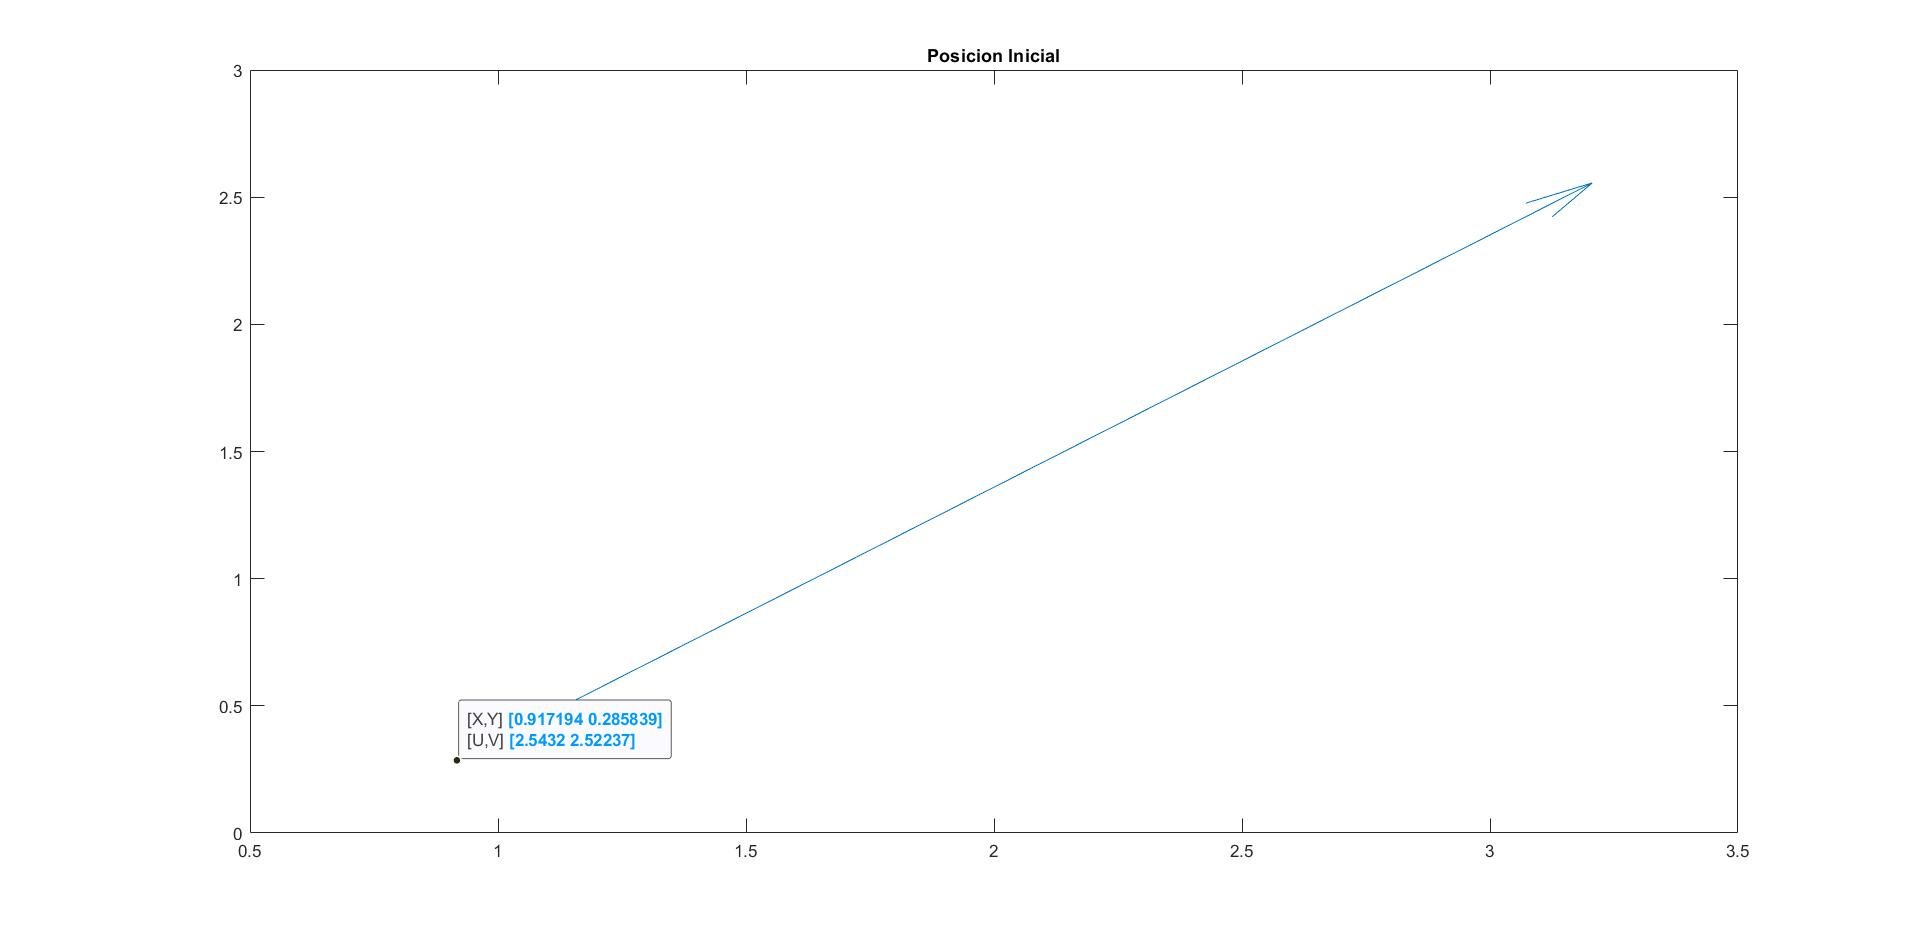
\includegraphics[scale=0.2]{fig/cap04/unelemento.jpg}
  \caption{Posición y velocidad inicial de un agente}
  \label{fig:posInicial}
\end{figure}


El comportamiento de este vector velocidad será el objeto de nuestro estudio en las próximas secciones. 
\subsection{Aplicación de los modelos}\label{s4_2_2}
En cada iteración pasa lo siguiente:
\begin{itemize}
    \item Se provee a cada modelo de una matriz de 20x4 con las posiciones y velocidades de todos los elementos (ver código fuente \ref{src:comparativa} 1-37).
    \item A esos datos se les aplica el modelo de consenso correspondiente. Las funcionen desarrolladas pueden verse en los anexos \ref{src:cs0}, \ref{src:csarbor}, \ref{src:cstrelat1}, \ref{src:cstrelat2}
    \item El modelo devuelve otra matriz 20x4 con los datos modificados (\ref{src:comparativa} 34-37, 50-53)
    \item Se guarda en una lista las diferencias de velocidades en cada iteración en cada modelo. (\ref{src:comparativa} 61, \ref{src:maxdif})
    \item Se representan las nuevas posiciones y velocidades de los 20 individuos en las n gráficas diferentes de los modelos a comparar(\ref{src:comparativa} 64-95)
\end{itemize}

\subsection{Comparativa y gráficas de simulación de comportamiento}\label{s4_2_3}
Durante toda la ejecución, se observa en una gráfica cómo se modifica en cada iteración el movimiento de cada elemento. 
Una vez finalizada la ejecución, se representan en otra gráfica cómo han cambiado los vectores velocidad a lo largo del tiempo en cada modelo gracias a la lista que se ha ido guardando de la media de las diferencias del vector velocidad. 

\begin{figure}[h]
  \centering
    \includesvg[scale=0.2]{fig/cap04/elementos.svg}
  \caption{Comportamiento de cada modelo}
\end{figure}

\subsection{Diferencia máxima de velocidad}\label{s4_2_4}
Aunque visualmente en las pruebas se puede ver cómo los vectores poco a poco tienden a una dirección común, notar esto en cada iteración es complicado y por ello se va a ir obteniendo una gráfica de la diferencia máxima que existe en un momento dado con respecto a la media del grupo según la ecuación \ref{eq:vmax}.

\begin{equation}\label{eq:vmax}
    \begin{array}{l}
        v_{max} = \displaystyle{\max\left(\|v_{i}-\frac{1}{N}\sum_{j=0}^{N}\vec{v_{j}}\|\right)}
    \end{array}
    \begin{array}{r}
        (i= 0, ..., N)
    \end{array}
\end{equation}

En las gráficas que representan la evolución de este dato a lo largo de la ejecución el eje de ordenadas es relativo a la máxima diferencia de todo el grupo y el eje de abscisas representa el tiempo en milisegundos.

\section{Modelo general de Cucker Smale} \label{s4_3}
Antes de mostrar gráficamente cómo afecta la aplicación de un modelo de control a Cucker-Smale y de comparar los diferentes controles propuestos por los autores vistos en el capítulo anterior, es necesario comprender cómo el modelo general de Cucker-Smale afecta al vector velocidad de cada uno de los individuos que conforman un grupo de animales, ya sea una bandada de pájaros, un banco de peces o cualquier animal social de los vistos con anterioridad. 

Las pruebas sobre este modelo se hacen en función del parámetro $\beta$ que como ya se ha comentado, la condición indispensable para que se llegue al consenso, es que tenga un valor $\beta \leq 1/2$. A continuación mostramos dos casos generales con dos valores de $\beta$ diferentes.

\subsection{Caso 1: se llega al consenso} \label{s4_3_1}
Para demostrar cómo aplicando el modelo de Cucker-Smale se llega al consenso, se elige una $\beta = 0.25$. 

\begin{figure}[htbp]
\centering
    \subcaptionbox{Posición inicial\label{fig:pos-i}}{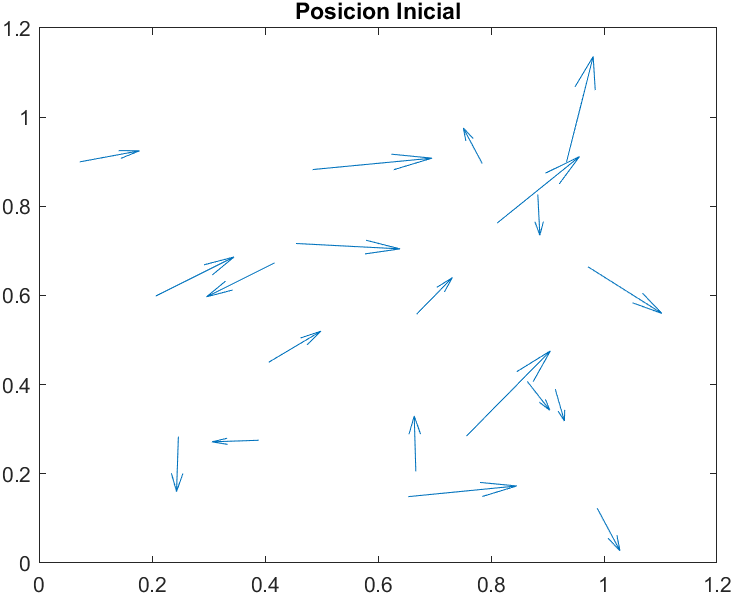
\includegraphics[height=5.5cm]{fig/cap04/1CSB025/posicion_inicial.png}}
    \subcaptionbox{Posición final\label{fig:pos-f}}{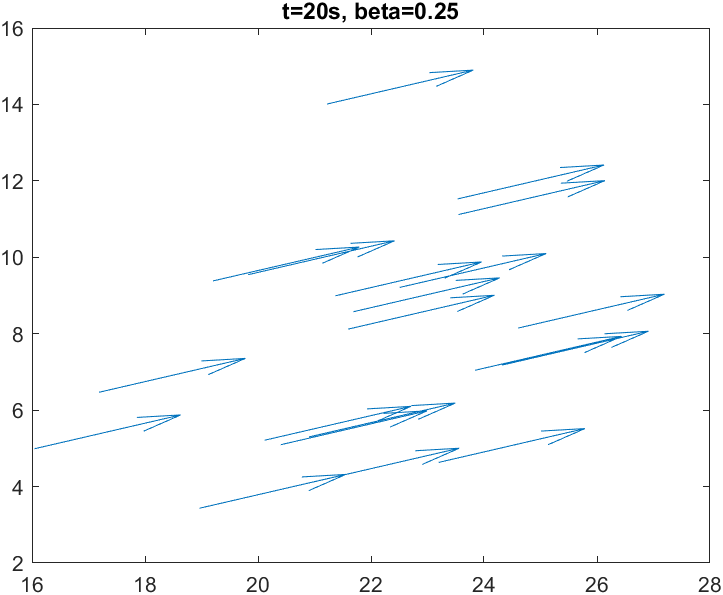
\includegraphics[height=5.5cm]{fig/cap04/1CSB025/posicion_final.png}}
\caption{Evolución del grupo en un tiempo t=20s} 
\label{fig:CS025_pos}
\end{figure}

Esta simulación se ha hecho utilizando un tiempo de 20s y se puede observar en las figuras (fig. \ref{fig:CS025_pos}) como partiendo de una posición y velocidades totalmente aleatorias en el espacio, todos los vectores han terminado convergiendo hacia el mismo. En la figura \ref{fig:CS025_vel} obtenemos una gráfica en la que se ve cómo con el paso del tiempo, la diferencia entre el vector más alejado es menor con respecto a la media de los demás. 
\begin{figure}
    \centering
    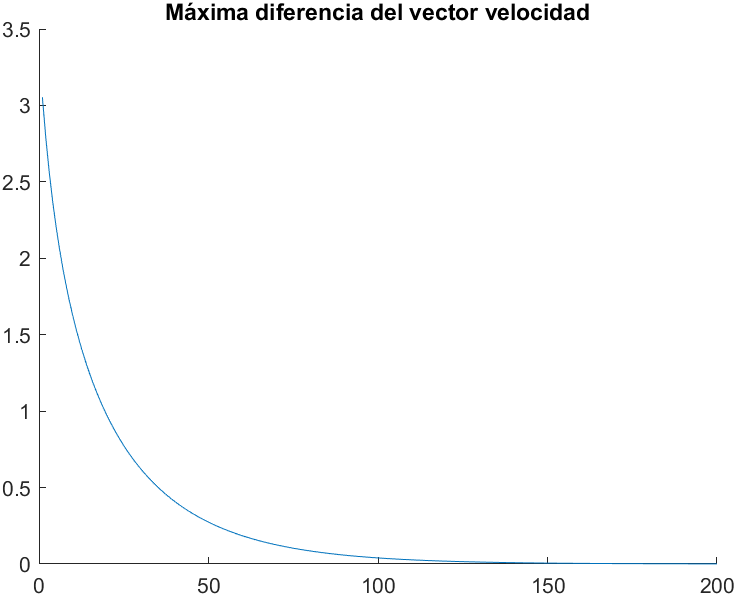
\includegraphics[height=5.5cm]{fig/cap04/1CSB025/velocidad.png}
    \caption{Evolución de la diferencia de velocidades}
    \label{fig:CS025_vel}
\end{figure}

Según los datos, en el segundo 20 la máxima diferencia de la velocidad de un elemento con respecto a la media sigue existiendo ($\|\vec{v_i}\|-\|\Bar{v}\| \approx 0.0010$) y para poder disminuir este valor se han hecho otras simulaciones aumentando el tiempo de ejecución, llegando  a obtener una diferencia $\|\vec{v_i}\|-\|\Bar{v}\| \approx 3.1451\cdot10^{-8}$ en un tiempo de simulación de $t=60s$. Esto muestra que esta diferencia tiende a 0 y además el ratio de decaimiento es significativo con una configuración del parámetro de convergencia $\beta\leq0.5$, tal y como dicen Cucker y Smale en su estudio. 

\subsection{Caso 2: se produce la dispersión} \label{s4_3_2}
Para demostrar cómo aplicando el modelo de Cucker-Smale el grupo se dispersa, se elige un valor del parámetro $\beta = 0.75$ obteniendo con cualquiera de las simulaciones, un resultado final similar al que se muestra en la figura \ref{fig:CS075_pos}.

\begin{figure}[htbp]
\centering
    \subcaptionbox{Posición inicial\label{fig:pos-i-075}}{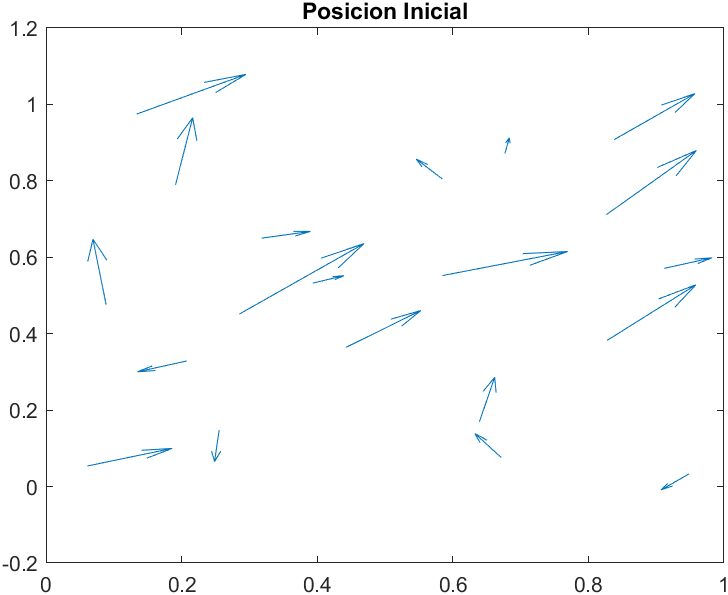
\includegraphics[height=5.5cm]{fig/cap04/2CSB075/posicion_inicial.png}}
    \subcaptionbox{Posición final\label{fig:pos-f-075}}{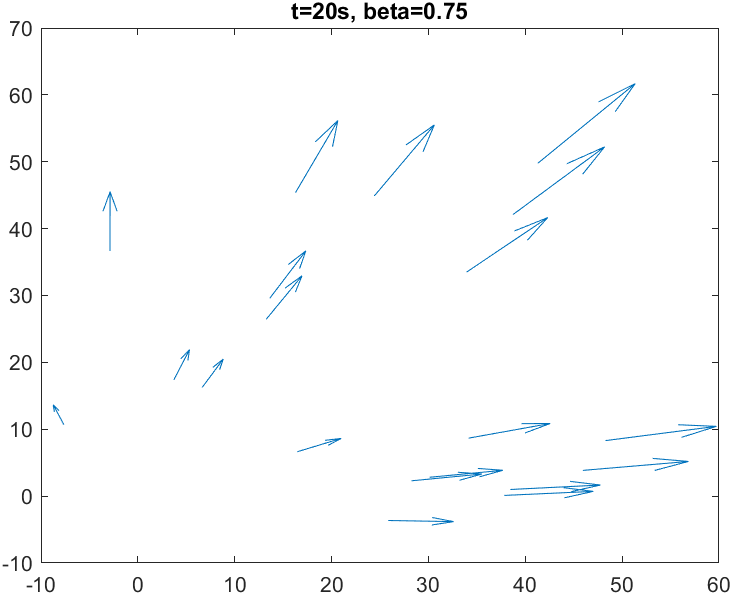
\includegraphics[height=5.5cm]{fig/cap04/2CSB075/posicion_final.png}}
\caption{Evolución del grupo en un tiempo t=20s} 
\label{fig:CS075_pos}
\end{figure}

Se han realizado adicionalmente varias ejecuciones, cada una con diferentes tiempos de simulación, para asegurarse de que los vectores de velocidad nunca llegan al consenso tendiendo a un valor que nunca es 0 para diferentes tiempos finitos (ver fig. \ref{fig:CS075_vel}) aunque no se puede determinar si las curvas tienden a un valor positivo o a cero, a un ritmo cada cada vez más lento en el tiempo, lo que es compatible con el teorema de Cucker Smale que dice que con una $\beta>0.5$ siempre se puede producir el consenso del grupo en un tiempo infinito, si se dan las condiciones iniciales adecuadas.

\begin{figure}[htbp]
\centering
    \subcaptionbox{t=20}{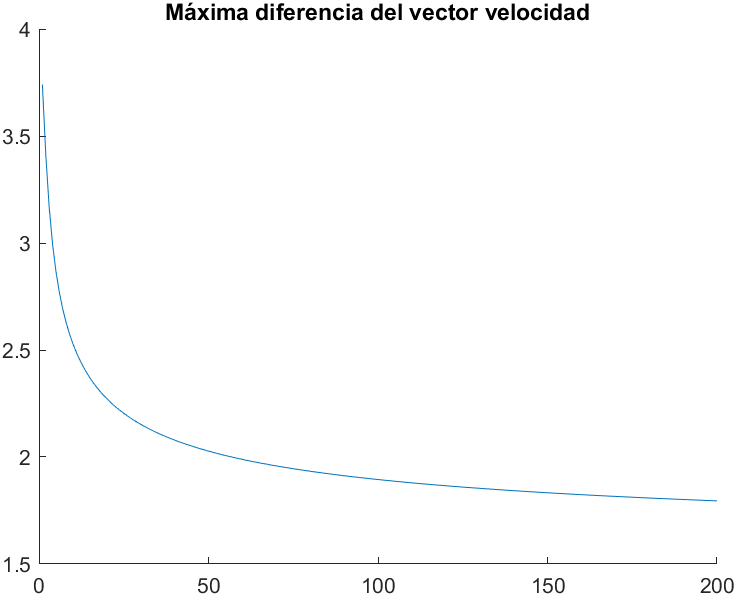
\includegraphics[height=5.5cm]{fig/cap04/2CSB075/velocidad20s.png}}
    \subcaptionbox{t=60(1)}{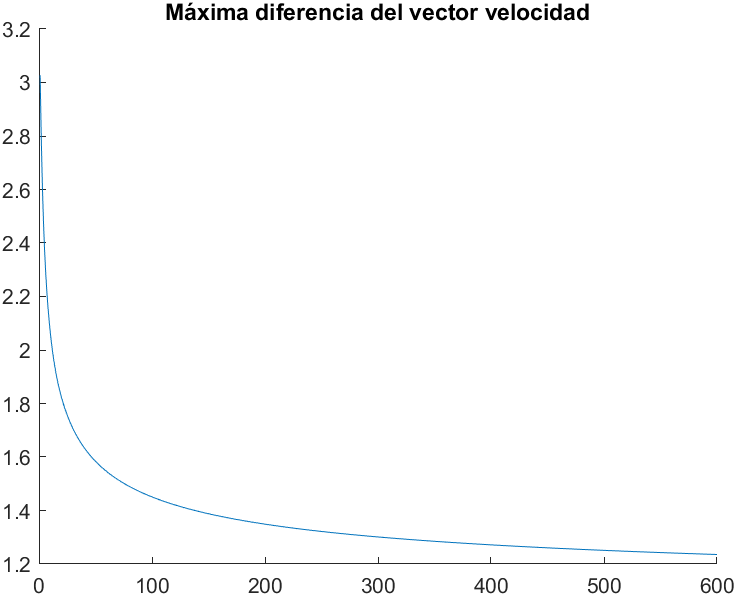
\includegraphics[height=5.5cm]{fig/cap04/2CSB075/velocidad60s1.png}}
    \subcaptionbox{t=60(2)}{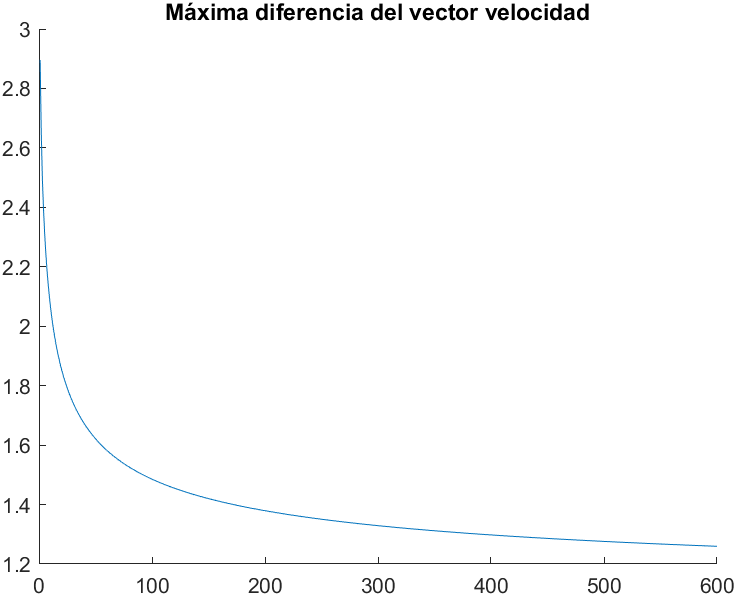
\includegraphics[height=5.5cm]{fig/cap04/2CSB075/velocidad60s2.png}}
    \subcaptionbox{t=120}{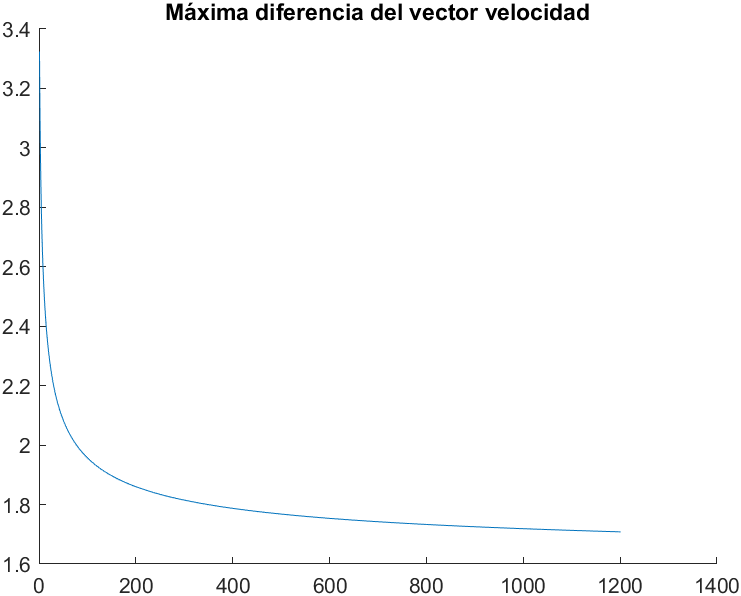
\includegraphics[height=5.5cm]{fig/cap04/2CSB075/velocidad120s.png}}
\caption{Evolución de la diferencia de velocidades con $\beta=0.75$} 
\label{fig:CS075_vel}
\end{figure}

Otra simulación que se ha hecho es minimizar la diferencia de los vectores velocidad de todos los miembros para generar una condición bajo la cual se llegue al consenso con un \linebreak $\beta > 0.75$ (figura \ref{fig:CS075_consenso}) pudiéndose observar y analizar desde dos puntos de vista. Por una parte, en la figura \ref{fig:CS075_consenso} se muestra que cuando la diferencia de estos vectores es suficientemente pequeña ($\pm 30^o$ en la dirección de los vectores), se llega al consenso. 

Por otra parte, teniendo en cuenta la figura \ref{fig:CS075_comparacion_consenso} también se puede observar cómo a medida que aumenta la diferencia inicial de estos vectores, el estado de consenso tarda más en producirse, hasta llegar a un punto en el que la diferencia es demasiado grande como para que se pueda producir la alineación del vector velocidad en un tiempo finito en el que pueda realizarse la simulación.

\begin{figure}[htbp]
\centering
    \subcaptionbox{Posición inicial}{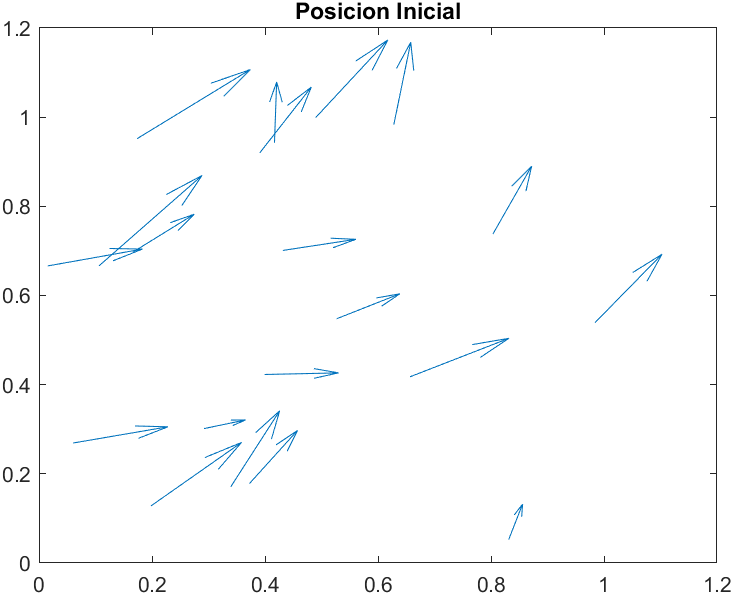
\includegraphics[height=5.5cm]{fig/cap04/2CSB075/consenso/posicion0102.png}}
    \subcaptionbox{Posición final}{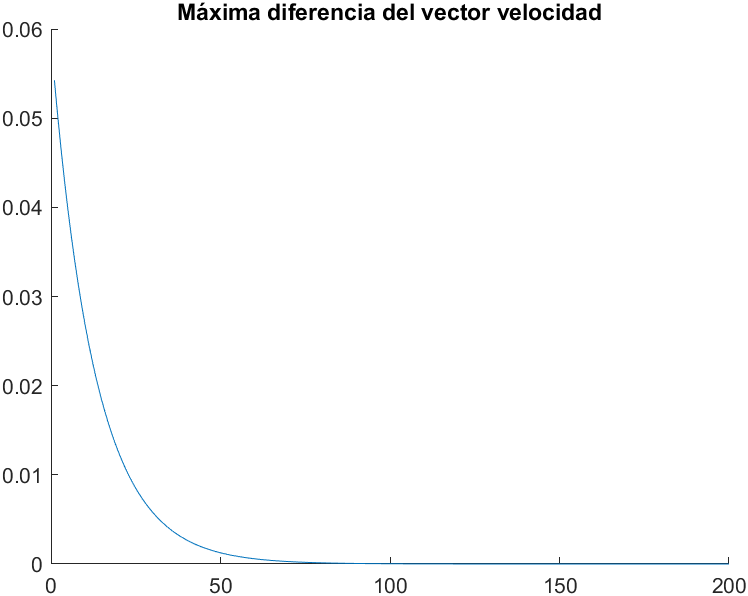
\includegraphics[height=5.5cm]{fig/cap04/2CSB075/consenso/velocidad0102.png}}
\caption{Consenso con una $\beta > 0.5$} 
\label{fig:CS075_consenso}
\end{figure}

\begin{figure}[!ht]
    \centering
    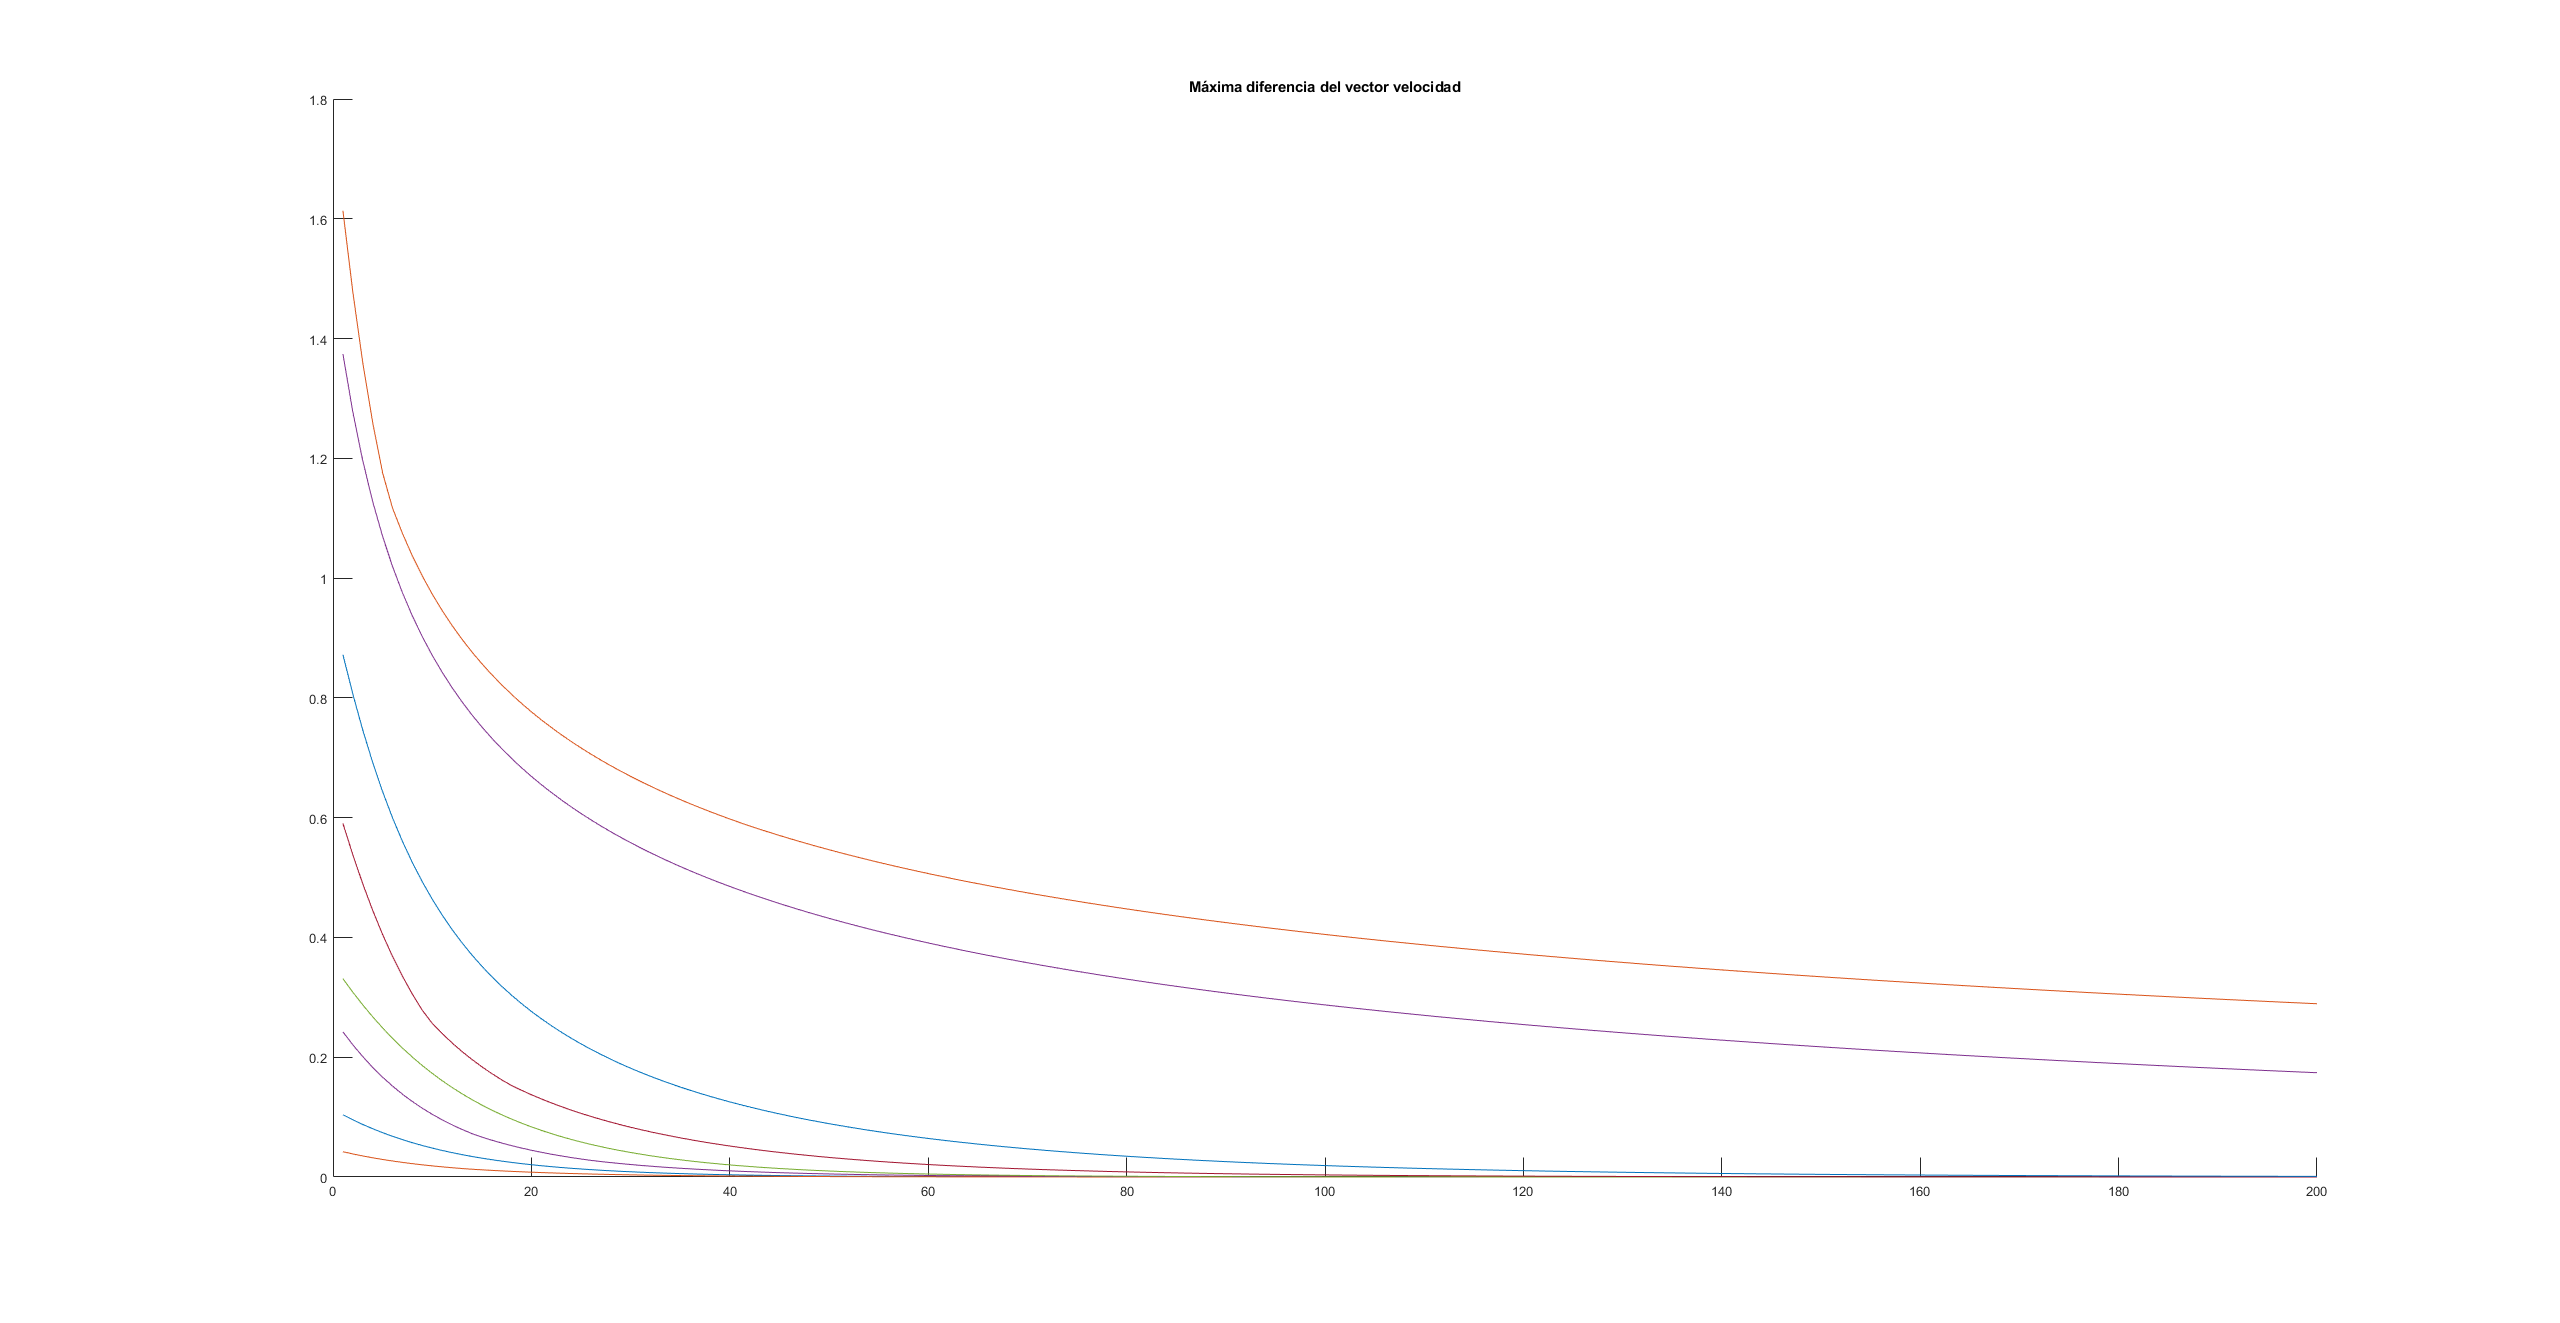
\includegraphics[width=\textwidth]{fig/cap04/2CSB075/consenso/todas.png}
    \caption{Comparación del comportamiento con respecto a la diferencia inicial cuando $\beta > 0.5$}
    \label{fig:CS075_comparacion_consenso}
\end{figure}

%\newpage
%\clearpage

\section{Aplicación de controles al modelo general de Cucker-Smale} \label{s4_4}

Una vez analizado y probado el modelo de Cucker Smale de manera práctica, se añaden a ese modelo los controles que se han visto en el capítulo anterior. Por una parte, se añade el control de CCR añadiendo su simulación a la gráfica y por otra parte se añaden dos controles diferentes basados en el modelo de Trelat, para poder comparar también cuál es la diferencia entre controlar todos los elementos a la vez dando un pequeño empujón a todos y modificar de forma más agresiva el más alejado, proporcionando el empujón únicamente a ese vector. 

En todo este capítulo se entiende que el grupo ha llegado al consenso cuando la diferencia máxima de velocidad sea inferior o igual a $0.01$.

\subsection{Comparación entre modelos en una ejecución}
En una primera ejecución aislada, se pretende comparar los 4 modelos diferentes y el comportamiento de los elementos $N=20$ durante un tiempo finito $t=20s$ con un valor de $\beta$ que facilite el consenso en todos los casos, $\beta=0.25$.

Tal y como se ha comentado en la sección \ref{s4_2_1}, se parte de una posición y dirección aleatoria de todos los elementos pero igual entre los 4 modelos tal y como se muestra en la figura \ref{fig:pos_inicial_4models}.

\begin{figure}[!h]
    \centering
    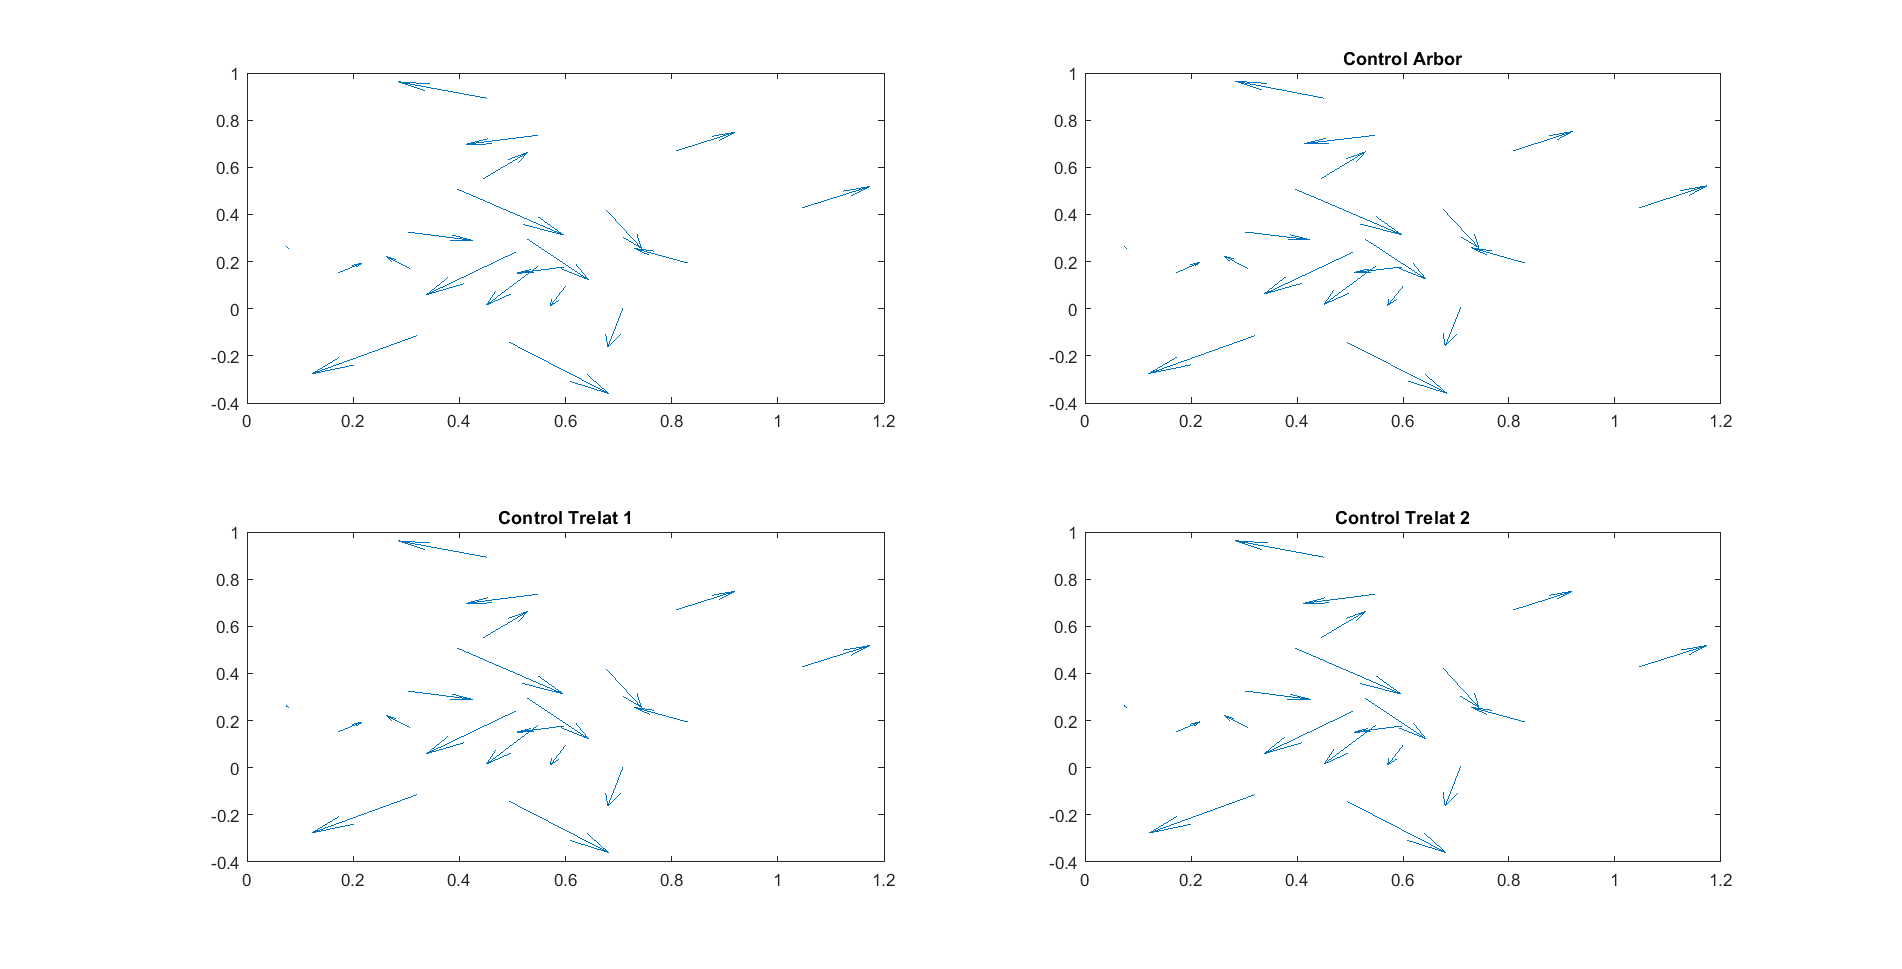
\includegraphics[width=\textwidth]{fig/cap04/3ALLB025/pos_inicial.png}
    \caption{Posición inicial de los 4 modelos.}
    \label{fig:pos_inicial_4models}
\end{figure}

Pasados los 20 segundos de ejecución, el estado de los individuo termina siendo el que se muestra en la figura \ref{fig:pos_final_4models} pudiendo observarse que los 4 modelos han conseguido llegar a una dirección común con la configuración inicial explicada.

\begin{figure}[h!]
    \centering
    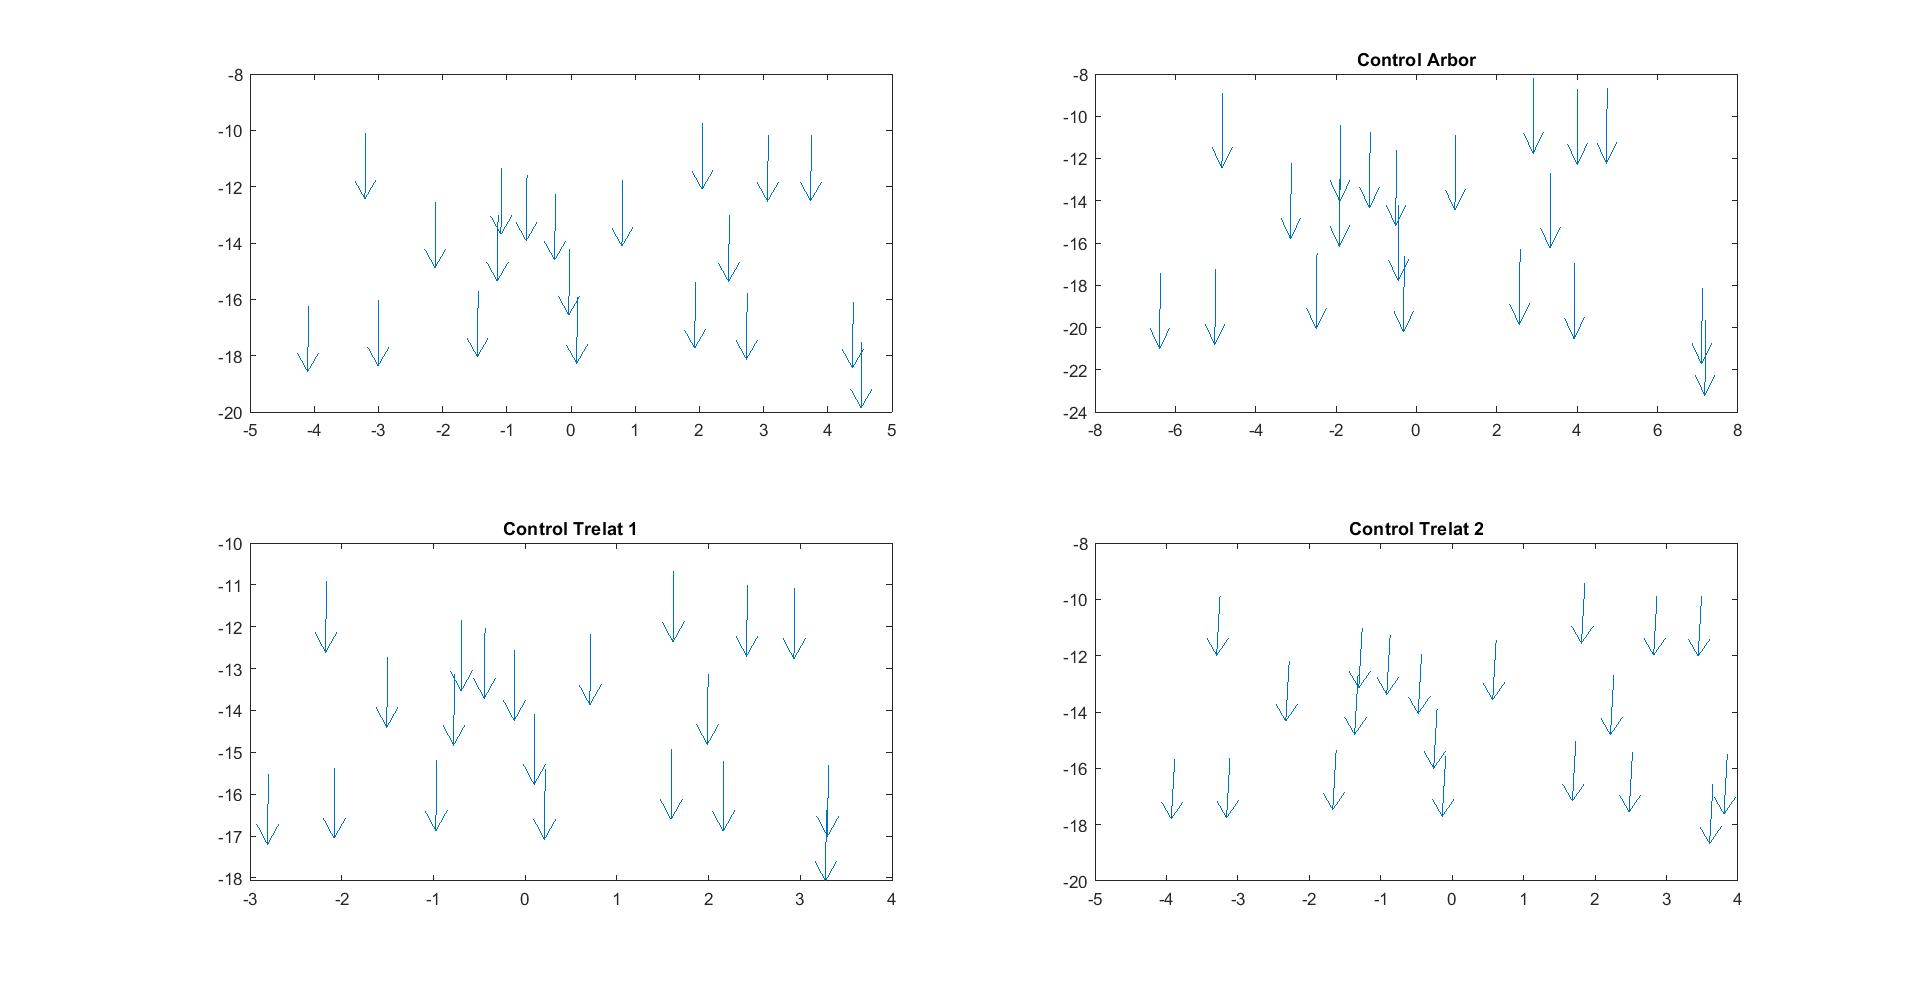
\includegraphics[width=\textwidth]{fig/cap04/3ALLB025/pos_final.png}
    \caption{Posición final de consenso de los 4 modelos.}
    \label{fig:pos_final_4models}
\end{figure}

Para poder hacer un estudio más exhaustivo del comportamiento en el tiempo de los 4 casos, en cada iteración se ha almacenado la máxima diferencia que hay entre todos los vectores en cada uno de los casos tal y como se ha explicado en la sección \ref{s4_2_4} de este mismo capítulo. 

Con estos datos se pretende obtener una gráfica que pueda comparar a qué velocidad se llega al consenso.

\begin{figure}[htbp]
\centering
    \subcaptionbox{Velocidad de consenso}{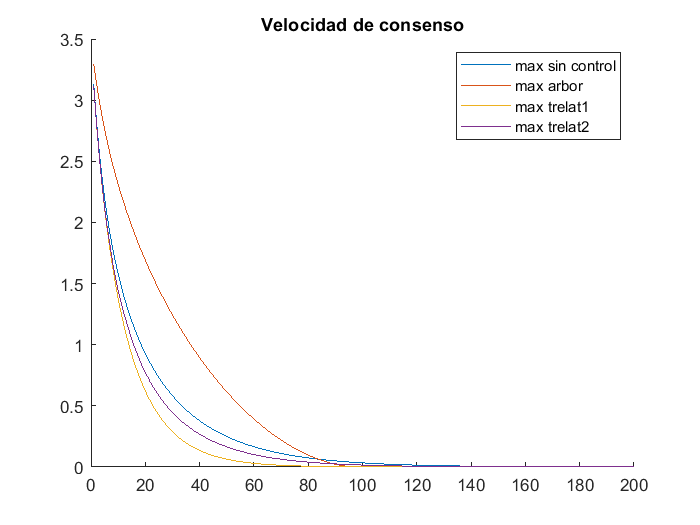
\includegraphics[height=5cm]{fig/cap04/3ALLB025/vel_consenso.png}}
    \subcaptionbox{Velocidad de consenso final ampliada}{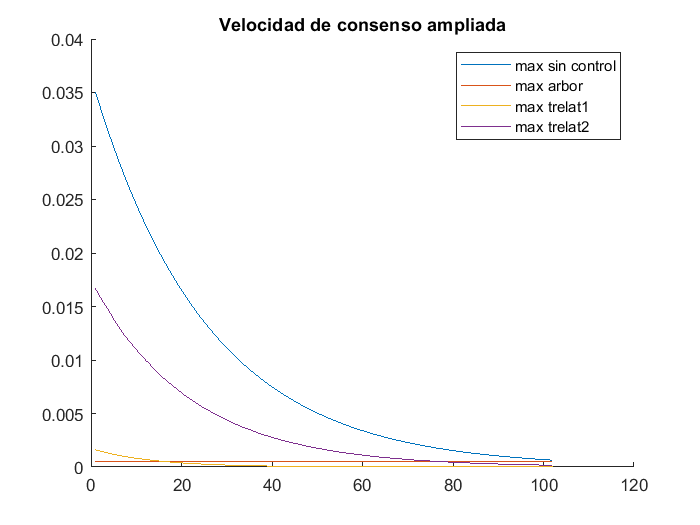
\includegraphics[height=5cm]{fig/cap04/3ALLB025/vel_consenso_ampliada.png}}
\caption{Comparación de la velocidad a la que se adquiere el consenso con $\beta = 0.25$.} 
\label{fig:consenso_4models}
\end{figure}

Un primer vistazo a la figura \ref{fig:consenso_4models}(a) sirve para corroborar que los 4 modelos terminan llegando al consenso en el tiempo fijado, con la diferencia de que cada uno lo hace a una velocidad diferente. Si se amplia la gráfica a los momentos finales donde parece que todos los modelos llegan al consenso (figura \ref{fig:consenso_4models}(b)) se puede analizar mejor qué ha sucedido en cada caso pudiendo así sacar varias conclusiones:

\begin{enumerate}
    \item El modelo de Cucker Smale sin ningún tipo de control añadido, es el último en llegar al consenso.
    \item El control que se propone en CCR, es el que tiene menos pendiente en la velocidad de consenso y el que antes llega (se puede ver en la gráfica ampliada que cuando Cucker Smale, y los dos de Trelat están todavía disminuyendo su máxima diferencia, el modelo de CCR ya ha llegado al consenso. 
    \item Entre los dos de Trelat, ambos llegan al consenso aunque Trelat2, que tiene menos gasto energético a la hora de controlar el modelo de CS, tarda más en obtener el estado de consenso.
\end{enumerate}

Se corrobora pues, gracias a estas simulaciones, que bajo las mismas condiciones iniciales y con una $\beta = 0.25$ todos los modelos llegan al consenso para un tiempo finito $t=20s$ habiendo una clara mejora cuando se aplica algún tipo de control sobre el modelo de Cucker Smale.

Si concluimos esta prueba configurando una $\beta=0.75$ y $t=120s$ entonces obtenemos que en el tiempo finito establecido los dos modelos que son capaces de obtener el consenso son los dos de Trèlat según la gráfica de la figura \ref{fig:consenso_4models_b075} mientras que Cucker Smale y CCR no lo han logrado en ese tiempo, aunque sí que lo harían si pudiera simularse un tiempo infinito.

\begin{figure}[htbp]
\centering
    \subcaptionbox{Velocidad de consenso}{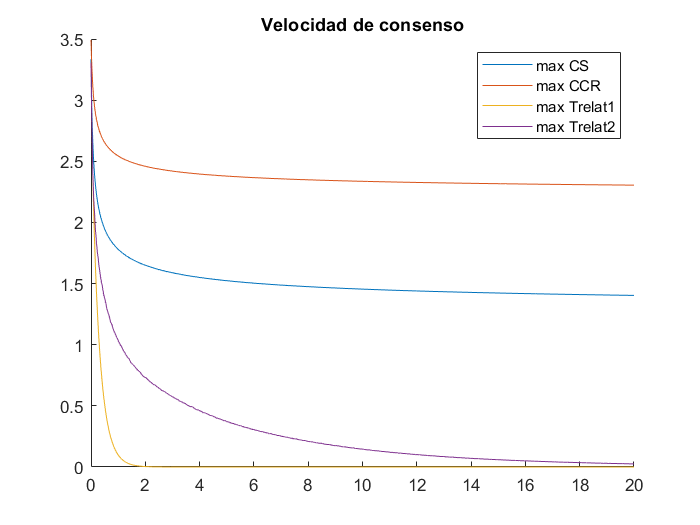
\includegraphics[height=5cm]{fig/cap04/4ALLB075/velocidad.png}}
    \subcaptionbox{Velocidad de consenso final ampliada}{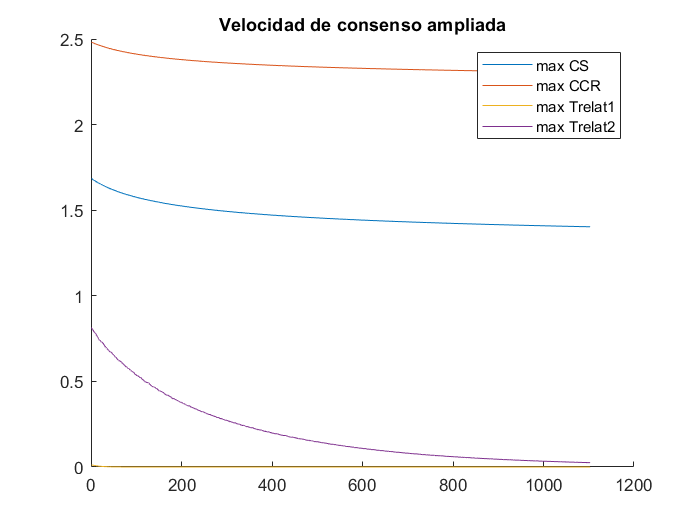
\includegraphics[height=5cm]{fig/cap04/4ALLB075/velocidad_ampliada.png}}
\caption{Comparación de la velocidad a la que se adquiere el consenso con $\beta=0.75$.} 
\label{fig:consenso_4models_b075}
\end{figure}

\subsection{Comparación entre ejecuciones}

Para descartar que los resultados obtenidos anteriormente sean objeto del azar y de una configuración específica del estado inicial del grupo, es necesario repetir esas pruebas una cantidad suficiente de veces cambiando las condiciones iniciales para obtener una media de datos que corroboren lo anterior.

Para ello se ha decidido comparar el momento en el que se llega al consenso partiendo de 500 posiciones iniciales diferentes. Es necesario aclarar en este punto, que al igual que en la sección anterior, se ha tomado la decisión de definir el momento en el que se considera que el grupo ha llegado al consenso, cuando la diferencia del módulo del vector más alejado con respecto a la media de la dirección del grupo, es igual o menor que $0.01$, es decir, $||v_{max}||$.

\begin{table}[!ht]
\caption{Tiempos de consenso en 500 ejecuciones con $\beta=0.25$ y $t=20s$}
    \centering
    \begin{tabular}{|l|l|l|l|l|}
    \hline
        \textbf{Nº Ejecución} & \textbf{$T_c$ CS} & \textbf{$T_c$ CCR} & \textbf{$T_c$ Trelat 1} & \textbf{$T_c$ Trelat 2} \\ \hline
        1 & 14 & 10,1 & 7,5 & 11,9 \\ \hline
        2 & 13,8 & 9,7 & 7,6 & 10,9 \\ \hline
        3 & 14,6 & 10 & 7,6 & 11,7 \\ \hline
        4 & 13,3 & 9,2 & 7,4 & 11,4 \\ \hline
        5 & 15,6 & 12,2 & 7,9 & 12,9 \\ \hline
        6 & 14,6 & 11 & 7,7 & 12,2 \\ \hline
        7 & 15,3 & 11 & 7,8 & 11,6 \\ \hline
        8 & 15,5 & 11,9 & 7,9 & 12 \\ \hline
        9 & 13,2 & 9 & 7,4 & 10,9 \\ \hline
        10 & 13,3 & 9 & 7,4 & 10,9 \\ \hline \hline
        ... & ... & ... & ... & ...\\ \hline \hline
        497 & 13,9 & 9,6 & 7,5 & 11,2 \\ \hline
        498 & 15,5 & 11,5 & 7,8 & 12,7 \\ \hline
        499 & 14,9 & 11,2 & 7,7 & 12,7 \\ \hline
        500 & 15,2 & 11,7 & 7,8 & 11,4 \\ \hline \hline
        \textbf{Promedio} & \textbf{14,4586} & \textbf{10,8066} & \textbf{7,6586} & \textbf{11,7518} \\ \hline
    \end{tabular}
    \label{tab:tiemposConsenso}
\end{table}

En la tabla \ref{tab:tiemposConsenso} se han cortado algunos resultados pero se puede observar claramente cuál es el modelo más efectivo para llegar antes al consenso, siendo el de Trèlat que impulsa en en cada iteración a todos sus elementos. Esto resulta coherente ya que este modelo impulsa a todos los elementos a la vez.

Se ha repetido el proceso anterior, llevando a cabo  500 repeticiones de la simulación, fijando el valor del parámetro $\beta$ en  $\beta=0.5$. En este caso ha sido necesario ampliar el tiempo de ejecución a $t=60s$. En este caso es curioso observar cómo por un lado el modelo de Cucker Smale sin aplicarle ningún control sólo consigue el consenso del grupo en 2 ocasiones mientras que el primer modelo de Trélat si que lo consigue en todas las ejecuciones. En la tabla \ref{tab:tiemposConsensoB05} se muestran algunos de los resultados obtenidos en esta prueba, entre los que se encuentran los más característicos:

\begin{table}[!h]
\caption{Tiempos de consenso en 500 ejecuciones con $\beta=0.5$ y $t=60s$}
    \centering
    \begin{tabular}{|l|l|l|l|l|}
    \hline
        \textbf{Nº Ejecución} & \textbf{$T_c$ CS} & \textbf{$T_c$ CCR} & \textbf{$T_c$ Trelat 1} & \textbf{$T_c$ Trelat 2} \\ \hline
        5 & 60 & 60 & \cellcolor{green!15}9,6 & \cellcolor{green!15}44,2 \\ \hline
        6 & 60 & 60 & \cellcolor{green!15}9,9 & 60 \\ \hline \hline
        11 & 60 & 60 & \cellcolor{green!15}9,5 & \cellcolor{green!15}41,8 \\ \hline
        12 & \cellcolor{green!15}51,8 & \cellcolor{green!15}38,1 & \cellcolor{green!15}8,4 & \cellcolor{green!15}23,4 \\ \hline \hline
        58 & 60 & 60 & \cellcolor{green!15}9,6 & \cellcolor{green!15}50,3 \\ \hline
        59 & 60 & 60 & \cellcolor{green!15}9,8 & 60 \\ \hline \hline
        139 & 60 & 60 & \cellcolor{green!15}9,5 & \cellcolor{green!15}39,3 \\ \hline
        140 & 60 & 60 & \cellcolor{green!15}9,5 & 60 \\ \hline \hline
        216 & 60 & 60 & \cellcolor{green!15}9,6 & \cellcolor{green!15}50,3 \\ \hline
        217 & 60 & 60 & \cellcolor{green!15}9,5 & 60 \\ \hline \hline
        243 & 60 & 60 & \cellcolor{green!15}9,3 & \cellcolor{green!15}36,2 \\ \hline
        244 & 60 & 60 & \cellcolor{green!15}9,9 & 60 \\ \hline \hline
        290 & 60 & 60 & \cellcolor{green!15}9,3 & \cellcolor{green!15}38,6 \\ \hline
        291 & 60 & 60 & \cellcolor{green!15}9,6 & 60 \\ \hline \hline
        388 & 60 & 60 & \cellcolor{green!15}9,2 & \cellcolor{green!15}42,1 \\ \hline
        389 & 60 & 60 & \cellcolor{green!15}9,8 & 60 \\ \hline \hline
        440 & 60 & 60 & \cellcolor{green!15}8,9 & \cellcolor{green!15}28,8 \\ \hline
        441 & 60 & \cellcolor{green!15}55,2 & \cellcolor{green!15}8,6 & \cellcolor{green!15}31,2 \\ \hline \hline
        477 & 60 & 60 & \cellcolor{green!15}9,3 & \cellcolor{green!15}44,9 \\ \hline
        478 & \cellcolor{green!15}57,2 & \cellcolor{green!15}53,5 & \cellcolor{green!15}8,5 & \cellcolor{green!15}26,5 \\ \hline \hline
        499 & 60 & 60 & \cellcolor{green!15}9,3 & \cellcolor{green!15}50,6 \\ \hline
        500 & 60 & 60 & \cellcolor{green!15}8,8 & \cellcolor{green!15}41,3 \\ \hline \hline
        \textbf{Total} & \textbf{2} & \textbf{3} & \textbf{500} & \textbf{493} \\ \hline
    \end{tabular}
    \label{tab:tiemposConsensoB05}
\end{table}

Analizando los datos de la tabla puede observarse que en el caso de $\beta=0.5$, aunque los modelos de Cucker Smale y CCR solo hayan llegado al consenso en 2 y 3 ocasiones respectivamente, el segundo de ellos, consigue una menor dispersión de sus elementos.

Por último, se ha hecho una prueba con una $\beta=0.75$ y cambiando un poco código se ha pretendido realizar una ejecución eliminando el límite del tiempo de la ejecución, y simplemente definiendo el final de la ejecución cuando lo 4 modelos hayan llegado al estado que hemos definido de consenso. El resultado ha sido que los dos modelos de Trélat han conseguido el estado de consenso en un tiempo de 10s y 141s respectivamente, frente a los otros dos modelos que en un tiempo de 60 días no han logrado disminuir suficientemente la diferencia entre los vectores de dirección de sus elementos como para llegar al estado de consenso. Esto no quiere decir que no puedan llegar nunca, pues estos valores siguen disminuyendo a lo largo del tiempo a pesar de hacerlo de manera muy lenta.